%% Compétences : 4C07-GEO07, 4C07-GEO08, 4C07-GEO09
%% Cours (trace écrite copiée au tableau), d'après la brochure IREM de Paris n° 100,
%% « Enseigner la géométrie au cycle 4 », ch. 7 et 8 (extrait dans _Archive/).
%% Choix de la brochure : on définit les triangles semblables par les angles ET les côtés
%% (comme les polygones semblables) ; « deux angles suffisent » est une propriété.

%% Font size %%
\documentclass[11pt]{article}

%% Load the custom package
\usepackage{Mathdoc}
\usepackage{icomma}
\usepackage{colortbl}
\usetikzlibrary{angles,quotes,calc}

%% Numéro de séquence %% Titre de la séquence %%
\renewcommand{\centerhead}{S07 - Triangles semblables}

% Encadré « compétence » en tête de partie
\newcommand{\comp}[2]{\par\smallskip\noindent\colorbox{gray!15}{\parbox{\dimexpr\linewidth-2\fboxsep}{\small\textbf{Compétence #1} : #2}}\par\smallskip}
\newcommand{\f}[2]{\dfrac{#1}{#2}}
% Marques d'angles : un arc (rouge), deux arcs (bleu), trois arcs (vert)
\tikzset{
  a1/.style={draw=red!70!black, thick, angle radius=4mm},
  a2/.style={draw=blue!70!black, thick, angle radius=4mm, double, double distance=1pt},
  a3/.style={draw=green!50!black, thick, angle radius=5mm, fill=green!15},
}

%% Spacing commands %%
\renewcommand{\baselinestretch}{1} \setlength{\parindent}{0pt}

\begin{document}

\begin{tcolorbox}[colback=white,colframe=black,boxrule=0.6pt,arc=2mm,title={\textbf{Ce que je dois savoir faire à la fin du chapitre}},coltitle=black,colbacktitle=gray!15]
\begin{tabular}{@{}ll@{}}
\textbf{4C07-GEO07} & Reconnaître des triangles semblables : cas \textbf{ACA} \hfill (parties 3 et 4)\\
\textbf{4C07-GEO08} & Reconnaître des triangles semblables : cas \textbf{CCC} et \textbf{CAC} \hfill (parties 3 et 4)\\
\textbf{4C07-GEO09} & \textbf{Calculer des longueurs} avec des triangles semblables \hfill (partie 5)\\
\end{tabular}
\end{tcolorbox}

%% ------------------------------------------------------------------
\section{Des figures de même forme}

\begin{definition}
Deux polygones ont la \textbf{même forme} (on dit qu'ils sont \textbf{semblables}) lorsque l'un est un
\textbf{agrandissement} ou une \textbf{réduction} de l'autre :
\begin{itemize}
\item leurs angles sont \textbf{égaux} deux à deux ;
\item leurs côtés sont \textbf{proportionnels} : toutes les longueurs sont multipliées par un même nombre $k$.
\end{itemize}
$k$ est le \textbf{coefficient} : si $k > 1$, c'est un agrandissement ; si $k < 1$, c'est une réduction.
\end{definition}

\begin{minipage}{0.42\linewidth}
\begin{exemple}
Des rectangles de même forme : $2 \times 1,4$ ; \ $3 \times 2,1$ ; \ $4 \times 2,8$
(la largeur vaut toujours $0,7$ fois la longueur).\\
Posés dans le même angle droit, leurs \textbf{diagonales sont alignées}.
\end{exemple}
\end{minipage}\hfill
\begin{minipage}{0.55\linewidth}\centering
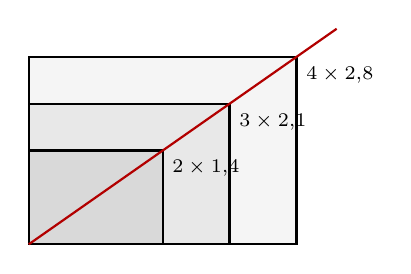
\begin{tikzpicture}[scale=0.85]
  \draw[thick, fill=gray!8] (0,0) rectangle (4,2.8);
  \draw[thick, fill=gray!18] (0,0) rectangle (3,2.1);
  \draw[thick, fill=gray!30] (0,0) rectangle (2,1.4);
  \draw[red!70!black, thick] (0,0) -- (4.6,3.22);
  \node[below right,font=\scriptsize] at (2,1.4) {$2\times1,4$};
  \node[below right,font=\scriptsize] at (3,2.1) {$3\times2,1$};
  \node[below right,font=\scriptsize] at (4,2.8) {$4\times2,8$};
\end{tikzpicture}
\end{minipage}

\begin{remarque}
Les deux conditions sont nécessaires. Un carré et un rectangle non carré ont les mêmes angles (droits)
mais pas la même forme ; un carré et un losange de même côté ont des côtés proportionnels mais pas la même forme.
\end{remarque}

%% ------------------------------------------------------------------
\section{Triangles semblables : définition et vocabulaire}

\begin{definition}
Deux triangles sont \textbf{semblables} lorsqu'ils ont leurs \textbf{trois angles égaux} deux à deux
et leurs \textbf{côtés proportionnels}.
\end{definition}

\begin{center}
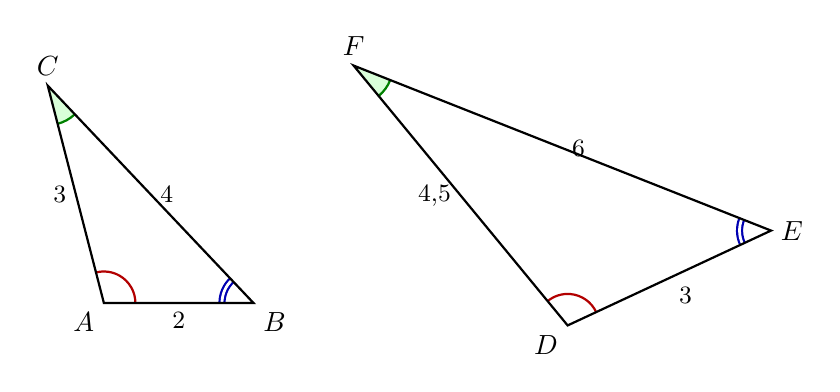
\begin{tikzpicture}[scale=0.95]
  % ABC : AB = 2, AC = 3, BC = 4
  \coordinate (A) at (0,0); \coordinate (B) at (2,0); \coordinate (C) at (-0.75,2.905);
  \pic[a1] {angle=B--A--C}; \pic[a2] {angle=C--B--A}; \pic[a3] {angle=A--C--B};
  \draw[thick] (A) -- (B) -- (C) -- cycle;
  \node[below left] at (A) {$A$}; \node[below right] at (B) {$B$}; \node[above] at (C) {$C$};
  \node[below,font=\small] at ($(A)!0.5!(B)$) {$2$};
  \node[left,font=\small] at ($(A)!0.5!(C)$) {$3$};
  \node[right,font=\small] at ($(B)!0.5!(C)$) {$4$};
  % DEF : agrandissement de coefficient 1,5, tourné
  \begin{scope}[shift={(6.2,-0.3)}, rotate=25, scale=1.5]
    \coordinate (D) at (0,0); \coordinate (E) at (2,0); \coordinate (F) at (-0.75,2.905);
  \end{scope}
  \pic[a1] {angle=E--D--F}; \pic[a2] {angle=F--E--D}; \pic[a3] {angle=D--F--E};
  \draw[thick] (D) -- (E) -- (F) -- cycle;
  \node[below left] at (D) {$D$}; \node[right] at (E) {$E$}; \node[above] at (F) {$F$};
  \node[below right,font=\small] at ($(D)!0.5!(E)$) {$3$};
  \node[left,font=\small] at ($(D)!0.5!(F)$) {$4,5$};
  \node[right,font=\small] at ($(E)!0.5!(F)$) {$6$};
\end{tikzpicture}
\end{center}

\begin{vocabulaire}
Dans deux triangles semblables, les sommets des angles égaux sont des \textbf{sommets homologues} ;
les côtés \textbf{opposés} aux angles égaux sont des \textbf{côtés homologues}.
\end{vocabulaire}

\begin{center}
\renewcommand{\arraystretch}{1.35}
\begin{tabular}{|c|c|c|}
\hline
\textbf{Sommets homologues} & \textbf{Angles égaux} & \textbf{Côtés homologues} \\ \hline
$A$ et $D$ & $\widehat{BAC} = \widehat{EDF}$ & $[BC]$ et $[EF]$ \\ \hline
$B$ et $E$ & $\widehat{ABC} = \widehat{DEF}$ & $[AC]$ et $[DF]$ \\ \hline
$C$ et $F$ & $\widehat{ACB} = \widehat{DFE}$ & $[AB]$ et $[DE]$ \\ \hline
\end{tabular}\\[3mm]
\begin{tabular}{|l|c|c|c|}
\hline
\textbf{Côtés de $ABC$} & $AB = 2$ & $AC = 3$ & $BC = 4$ \\ \hline
\textbf{Côtés de $DEF$} & $DE = 3$ & $DF = 4,5$ & $EF = 6$ \\ \hline
\multicolumn{4}{r}{coefficient $k = 1,5$ \ (agrandissement)}
\end{tabular}
\end{center}

%% ------------------------------------------------------------------
\section{Reconnaître des triangles semblables : les trois cas}
\comp{4C07-GEO07 et GEO08}{reconnaître des triangles semblables \hfill \textit{Fiches Ex-4C07-01 à 04}}

Pas besoin de tout vérifier : comme pour \textbf{construire un triangle} en 5\textsuperscript{e}, trois informations suffisent.
On note \textbf{A} pour un angle et \textbf{C} pour un côté.

\begin{center}
\renewcommand{\arraystretch}{1.3}
\begin{tabular}{|>{\centering\arraybackslash}m{5.2cm}|>{\centering\arraybackslash}m{5.2cm}|>{\centering\arraybackslash}m{5.2cm}|}
\hline
\textbf{Cas ACA} & \textbf{Cas CCC} & \textbf{Cas CAC} \\ \hline
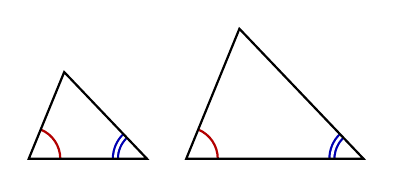
\begin{tikzpicture}[scale=0.5]
  \coordinate (A) at (0,0); \coordinate (B) at (3,0); \coordinate (C) at (0.9,2.2);
  \pic[a1] {angle=B--A--C}; \pic[a2] {angle=C--B--A};
  \draw[thick] (A) -- (B) -- (C) -- cycle;
  \begin{scope}[shift={(4,0)}, scale=1.5]
    \coordinate (D) at (0,0); \coordinate (E) at (3,0); \coordinate (F) at (0.9,2.2);
  \end{scope}
  \pic[a1] {angle=E--D--F}; \pic[a2] {angle=F--E--D};
  \draw[thick] (D) -- (E) -- (F) -- cycle;
\end{tikzpicture}
&
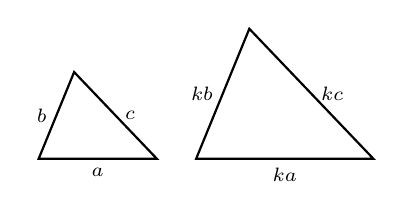
\begin{tikzpicture}[scale=0.5]
  \coordinate (A) at (0,0); \coordinate (B) at (3,0); \coordinate (C) at (0.9,2.2);
  \draw[thick] (A) -- (B) -- (C) -- cycle;
  \node[below,font=\scriptsize] at (1.5,0) {$a$}; \node[left,font=\scriptsize] at (0.45,1.1) {$b$}; \node[right,font=\scriptsize] at (1.95,1.1) {$c$};
  \begin{scope}[shift={(4,0)}, scale=1.5]
    \draw[thick] (0,0) -- (3,0) -- (0.9,2.2) -- cycle;
    \node[below,font=\scriptsize] at (1.5,0) {$k a$}; \node[left,font=\scriptsize] at (0.45,1.1) {$k b$}; \node[right,font=\scriptsize] at (1.95,1.1) {$k c$};
  \end{scope}
\end{tikzpicture}
&
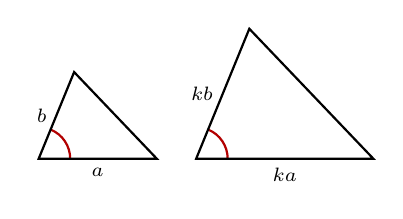
\begin{tikzpicture}[scale=0.5]
  \coordinate (A) at (0,0); \coordinate (B) at (3,0); \coordinate (C) at (0.9,2.2);
  \pic[a1] {angle=B--A--C};
  \draw[thick] (A) -- (B) -- (C) -- cycle;
  \node[below,font=\scriptsize] at (1.5,0) {$a$}; \node[left,font=\scriptsize] at (0.45,1.1) {$b$};
  \begin{scope}[shift={(4,0)}, scale=1.5]
    \coordinate (D) at (0,0); \coordinate (E) at (3,0); \coordinate (F) at (0.9,2.2);
    \node[below,font=\scriptsize] at (1.5,0) {$k a$}; \node[left,font=\scriptsize] at (0.45,1.1) {$k b$};
  \end{scope}
  \pic[a1] {angle=E--D--F};
  \draw[thick] (D) -- (E) -- (F) -- cycle;
\end{tikzpicture}
\\ \hline
\textbf{deux angles} égaux & \textbf{trois côtés} proportionnels & un \textbf{angle} égal \textbf{entre} deux côtés proportionnels \\ \hline
\small 5\textsuperscript{e} : construire un triangle avec un côté et les deux angles qui le touchent &
\small 5\textsuperscript{e} : construire un triangle avec ses trois côtés &
\small 5\textsuperscript{e} : construire un triangle avec deux côtés et l'angle entre eux \\ \hline
\end{tabular}
\end{center}

\begin{propriete}[Cas ACA]
Si deux triangles ont \textbf{deux angles égaux} deux à deux, alors ils sont semblables.
\end{propriete}
\par\medskip\noindent\hspace{0pt}
\par
\begin{remarque}
Le troisième angle est alors égal aussi (la somme des angles d'un triangle vaut $180\degre$).
Pour être \textbf{semblables}, la longueur du côté entre les deux angles n'a pas d'importance (pour être \textbf{égaux}, elle en a).
\end{remarque}

\begin{propriete}[Cas CCC]
Si les longueurs des \textbf{trois côtés} de deux triangles sont \textbf{proportionnelles}, alors ils sont semblables.
\end{propriete}
\par\medskip\noindent\hspace{0pt}
\par
\begin{exemple}[Méthode : ranger les longueurs dans l'ordre croissant, puis comparer les quotients]
$XYZ$ : $3$ ; $4,5$ ; $7,5$ \quad et \quad $MNO$ : $3,6$ ; $5,4$ ; $9$. \quad
$\f{3,6}{3} = \f{5,4}{4,5} = \f{9}{7,5} = 1,2$ : les triangles sont semblables ($k = 1,2$).\\
$XYZ$ et $DEF$ : $6$ ; $9,1$ ; $15$. \quad $\f{6}{3} = 2$ mais $\f{9,1}{4,5} \neq 2$ : ils ne sont \textbf{pas} semblables.
\end{exemple}

\begin{propriete}[Cas CAC]
Si deux triangles ont un \textbf{angle égal compris entre deux côtés proportionnels}, alors ils sont semblables.
\end{propriete}
\par\medskip\noindent\hspace{0pt}
\par
\begin{remarque}
\textbf{Attention :} l'angle doit être \textbf{entre} les deux côtés. Sinon, on ne peut pas conclure.\\
Tous les triangles équilatéraux sont semblables (cas ACA : leurs angles valent tous $60\degre$).
\end{remarque}

%% ------------------------------------------------------------------
\section{Les configurations à reconnaître}

\begin{center}
\renewcommand{\arraystretch}{1.2}
\begin{tabular}{|>{\centering\arraybackslash}m{3.7cm}|>{\centering\arraybackslash}m{3.7cm}|>{\centering\arraybackslash}m{3.7cm}|>{\centering\arraybackslash}m{3.7cm}|}
\hline
\textbf{Séparés, retournés} & \textbf{Emboîtés} & \textbf{Papillon} & \textbf{Angle commun, retourné} \\ \hline
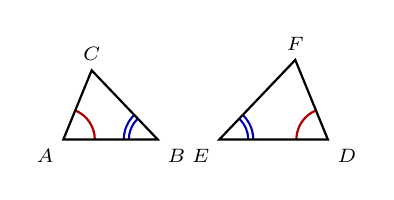
\begin{tikzpicture}[scale=0.4]
  \coordinate (A) at (0,0); \coordinate (B) at (3,0); \coordinate (C) at (0.9,2.2);
  \pic[a1] {angle=B--A--C}; \pic[a2] {angle=C--B--A};
  \draw[thick] (A) -- (B) -- (C) -- cycle;
  \node[below left,font=\scriptsize] at (A) {$A$}; \node[below right,font=\scriptsize] at (B) {$B$}; \node[above,font=\scriptsize] at (C) {$C$};
  \begin{scope}[shift={(8.4,0)}, xscale=-1.15, yscale=1.15]
    \coordinate (D) at (0,0); \coordinate (E) at (3,0); \coordinate (F) at (0.9,2.2);
  \end{scope}
  \pic[a1] {angle=F--D--E}; \pic[a2] {angle=D--E--F};
  \draw[thick] (D) -- (E) -- (F) -- cycle;
  \node[below right,font=\scriptsize] at (D) {$D$}; \node[below left,font=\scriptsize] at (E) {$E$}; \node[above,font=\scriptsize] at (F) {$F$};
\end{tikzpicture}
&
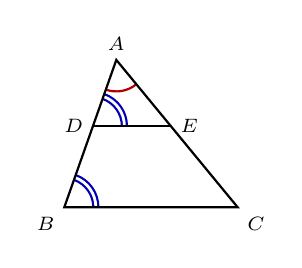
\begin{tikzpicture}[scale=0.55]
  \coordinate (A) at (1.2,3.4); \coordinate (B) at (0,0); \coordinate (C) at (4,0);
  \coordinate (D) at ($(A)!0.45!(B)$); \coordinate (E) at ($(A)!0.45!(C)$);
  \pic[a2] {angle=C--B--A}; \pic[a2] {angle=E--D--A}; \pic[a1] {angle=B--A--C};
  \draw[thick] (A) -- (B) -- (C) -- cycle; \draw[thick] (D) -- (E);
  \node[above,font=\scriptsize] at (A) {$A$}; \node[below left,font=\scriptsize] at (B) {$B$}; \node[below right,font=\scriptsize] at (C) {$C$};
  \node[left,font=\scriptsize] at (D) {$D$}; \node[right,font=\scriptsize] at (E) {$E$};
\end{tikzpicture}
&
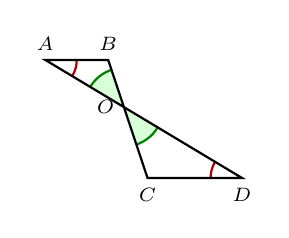
\begin{tikzpicture}[scale=0.5]
  \coordinate (O) at (2,1.4); \coordinate (A) at (0,2.6); \coordinate (B) at (1.6,2.6);
  \coordinate (C) at ($(O)!-1.5!(B)$); \coordinate (D) at ($(O)!-1.5!(A)$);
  \pic[a1] {angle=O--A--B}; \pic[a1] {angle=O--D--C};
  \pic[a3] {angle=B--O--A}; \pic[a3] {angle=C--O--D};
  \draw[thick] (A) -- (B) -- (C) -- (D) -- cycle;
  \node[above,font=\scriptsize] at (A) {$A$}; \node[above,font=\scriptsize] at (B) {$B$};
  \node[below,font=\scriptsize] at (C) {$C$}; \node[below,font=\scriptsize] at (D) {$D$};
  \node[left,font=\scriptsize] at (O) {$O$};
\end{tikzpicture}
&
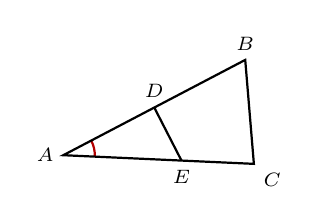
\begin{tikzpicture}[scale=0.55]
  \coordinate (A) at (0,0); \coordinate (B) at (4.2,2.2); \coordinate (C) at (4.4,-0.2);
  \coordinate (D) at ($(A)!0.5!(B)$); \coordinate (E) at ($(A)!0.62!(C)$);
  \pic[a1] {angle=C--A--B};
  \draw[thick] (A) -- (B) -- (C) -- cycle; \draw[thick] (D) -- (E);
  \node[left,font=\scriptsize] at (A) {$A$}; \node[above,font=\scriptsize] at (B) {$B$}; \node[below right,font=\scriptsize] at (C) {$C$};
  \node[above,font=\scriptsize] at (D) {$D$}; \node[below,font=\scriptsize] at (E) {$E$};
\end{tikzpicture}
\\ \hline
\small Je repère les sommets homologues \textbf{par les angles}, pas par la position.
&
\small $(DE) \parallel (BC)$ : angles \textbf{correspondants} égaux et angle $\widehat{A}$ commun \ $\to$ ACA.
&
\small $(AB) \parallel (CD)$ : angles \textbf{alternes-internes} et angles \textbf{opposés par le sommet} \ $\to$ ACA.
&
\small Angle $\widehat{A}$ commun et $\f{AD}{AC} = \f{AE}{AB}$ \ $\to$ CAC. \ Ici $D \leftrightarrow C$ et $E \leftrightarrow B$ !
\\ \hline
\end{tabular}
\end{center}

%% ------------------------------------------------------------------
\section{Calculer des longueurs}
\comp{4C07-GEO09}{calculer des longueurs avec des triangles semblables \hfill \textit{Fiches Ex-4C07-01 à 04}}

\begin{propriete}
Si deux triangles sont semblables, alors les longueurs de leurs \textbf{côtés homologues} sont proportionnelles.
\end{propriete}

\begin{minipage}{0.56\linewidth}
\begin{exemple}[Méthode]
Les triangles $ABC$ et $DEF$ ont $\widehat{A} = \widehat{D}$ et $\widehat{B} = \widehat{E}$.
\begin{enumerate}
\item Ils ont deux angles égaux : ils sont \textbf{semblables}.
\item Sommets homologues : $A$ et $D$, $B$ et $E$, $C$ et $F$.
\item Tableau des côtés homologues :
\end{enumerate}
\end{exemple}
\end{minipage}\hfill
\begin{minipage}{0.42\linewidth}\centering
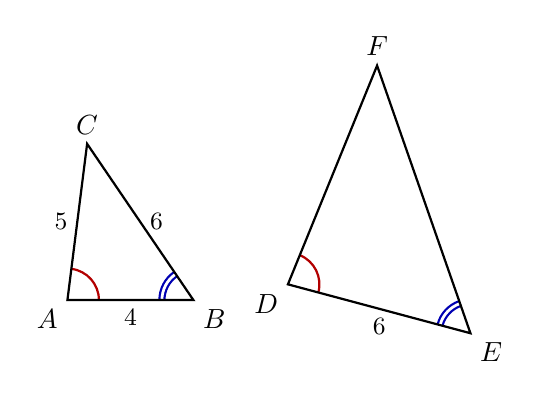
\begin{tikzpicture}[scale=0.4]
  \coordinate (A) at (0,0); \coordinate (B) at (4,0); \coordinate (C) at (0.625,4.961);
  \pic[a1] {angle=B--A--C}; \pic[a2] {angle=C--B--A};
  \draw[thick] (A) -- (B) -- (C) -- cycle;
  \node[below left] at (A) {$A$}; \node[below right] at (B) {$B$}; \node[above] at (C) {$C$};
  \node[below,font=\small] at ($(A)!0.5!(B)$) {$4$};
  \node[left,font=\small] at ($(A)!0.5!(C)$) {$5$};
  \node[right,font=\small] at ($(B)!0.5!(C)$) {$6$};
  \begin{scope}[shift={(7,0.5)}, rotate=-15, scale=1.5]
    \coordinate (D) at (0,0); \coordinate (E) at (4,0); \coordinate (F) at (0.625,4.961);
  \end{scope}
  \pic[a1] {angle=E--D--F}; \pic[a2] {angle=F--E--D};
  \draw[thick] (D) -- (E) -- (F) -- cycle;
  \node[below left] at (D) {$D$}; \node[below right] at (E) {$E$}; \node[above] at (F) {$F$};
  \node[below,font=\small] at ($(D)!0.5!(E)$) {$6$};
\end{tikzpicture}
\end{minipage}

\begin{center}
\renewcommand{\arraystretch}{1.4}
\begin{tabular}{|l|c|c|c|}
\hline
\textbf{Triangle $ABC$} & $AB = 4$ & $AC = 5$ & $BC = 6$ \\ \hline
\textbf{Triangle $DEF$} & $DE = 6$ & $DF = \ ?$ & $EF = \ ?$ \\ \hline
\end{tabular}
\qquad coefficient : $k = \f{DE}{AB} = \f{6}{4} = 1,5$
\end{center}
4. \ On multiplie par $k$ : \ $DF = 5 \times 1,5 = 7,5$ \qquad et \qquad $EF = 6 \times 1,5 = 9$.
\medskip

\begin{remarque}
\textbf{Attention aux sommets homologues} : le côté homologue de $[BC]$ est celui qui est \textbf{opposé} à l'angle
égal à $\widehat{A}$, c'est-à-dire $[EF]$, même si les triangles sont tournés ou retournés.
\end{remarque}

\end{document}

%%% Local Variables:
%%% mode: LaTeX
%%% TeX-master: t
%%% End:
